\chapter{Quadratic activation and initial conditions}
In this chapter, we introduce the first part of the original work of this thesis.
We further develop the framework introduced in previous chapters;
we will set an unusual activation function, but one that will allow us to derive
tractable equations for our purposes.

After that, we exhibit the code used for the simulation of the learning, and the differential
equation solution. 

Finally, we discuss the problem of the initial condition. Choosing the proper starting
point is one of the most challenging parts of this work. We briefly report our first
attempts to address the problem, leaving instead for the next chapter
the final choice.

\section{Quadratic activation function}
In the last chapter, we introduced the generic framework for studying soft committee machines.
We derived some generic differential equations, which, however, involve calculating an expectation value.
If the purpose is an analytical study of the process, it is necessary to find an explicit expression
for those values of expectation, otherwise, the study is arduous.

In previous literature\cite{saad1995line,goldt2019dynamics,veiga2022phase}, the standard choice in this case is
\[\sigma{(x)} = \erf{\left(\frac{x}{\sqrt{2}}\right)},\]
where \(\erf\) is the \emph{error function}. This choice is particularly convenient
because \(\erf\) is a regular and bound function, and its derivative is the gaussian.
The resulting expected values are computable; this is not clearly true for other 
common choices such as \emph{sigmoid} or \(\tanh\).

%todo: As an example, we report here what is Equation~\eqref{eq:genericODEforM} for this activation function.
Nevertheless, the expression obtained by computing the expected values in Equations~\eqref{eq:genericODE} involves
some inverse trigonometric functions, square roots and some other non-simple expressions. For reference, see
the Appendix~C of Veiga's paper\cite{veiga2022phase}, where the full expressions are reported.
Our ultimate goal is to derive analytical estimates of the learning times of the committee machines;
to do this we need the differential equations to be relatively simple and tractable with analytical techniques,
which unfortunately is not true with the canonical choice of \(\sigma\).
\begin{figure}
  \centering
  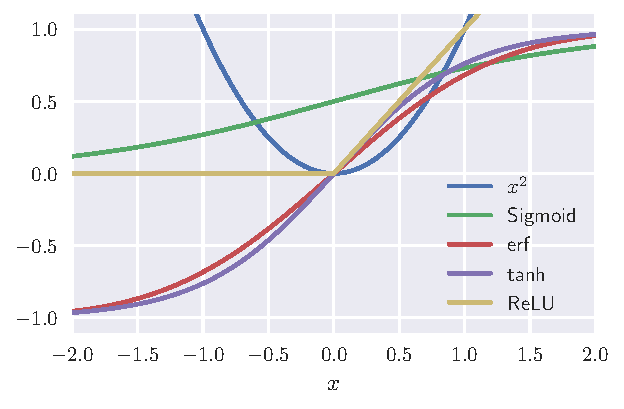
\includegraphics[width=0.7\textwidth]{figures/activation_function.pdf}
  \caption{ different choice of activation function.}
\end{figure}

Thus, the problem is now choosing a new activation function that would allow for more tractable equations.
The most natural choice is one with polynomial \(\sigma\). The simplest polynomial would be \(\sigma(x) = x\),
but it's well known that using a linear activation function in hidden layers leads to just a linear function,
so there is no point to use neural networks at all\cite{szandala2021review}\footnote{
  Actually, even if a deep neural network with linear activation is equivalent to a linear function, this does not mean that the dynamics of learning is the same as the corresponding function. See \cite{saxe2013exact} for reference. However, it is not of our interest to study the dynamics of a linear network.
}. 
Given all these considerations, the choice we did is \[\act{(x)} = x^2.\]
We need to point out a few things at this point.
First of all, the quadratic function, as well as all the other polynomial functions,
does not satisfies the Hypothesis~1 of Theorem~\ref{thm:process_to_ode_goldt}.
This seems to break the convergence of the differential equations solution to the
stochastic process of the training.
However, the fact that our condition violates the theorem does not necessarily imply that it is not true in this case. Following a discussion with the authors of the theorem, we have sufficient reason to believe that the proof can be extended to our activation function as well;
lipschitzianity was taken as a convenient assumption for the proof, but it is not the strictest condition we can have. We can also imagine truncating the parabola above a certain threshold, making the activation technically lipschitz.

Secondly, the usage of an even function as activation introduces an unusual symmetry in 
the functions. Both the student \(\hat{f}\) and the teacher \(f\) are even functions,
thus the sign of all the weights of a single neuron can be changed, without changing 
the output. In the macroscopic variables framework, this results in a loss of significance
of the sign of nondiagonal elements of \(\Q\) and \(\P\), and of all entries of \(\M\).
It follows that all these signs in the final state are determined by the choice of initial
conditions, and a small variation of those can lead to opposite solutions. This effect 
will mildly affect our analysis; we will point out this again when needed.

Finally, we notice that all the expected values we need to compute are just multivariate
polynomials of gaussian variables. The final result is particularly nice
because it is a polynomial in the covariance matrix entrances. The full derivation
is reported in Appendix~\ref{app:derivation-quadratic-ode}.
We report below the final expression of the equations.
\begin{subequations} \label{eq:quadraticODEs}\begin{align}
    \label{eq:quadraticODE_M}
    \dod{\M}{t} &= \frac{2 \gamma}{p}\left[
        \left(\frac{\Tr{\P}}k - \frac{\Tr{\Q}}p\right)\M +
        2\left(\frac{\M\P}{k} - \frac{\Q\M}{p}\right)
    \right] \\
    %
    \label{eq:quadraticODE_Q}
    \begin{split}
        \dod{\Q}{t} &= \frac{4 \gamma}{p}\left[
            \left(\frac{\Tr{\P}}k - \frac{\Tr{\Q}}p\right)\Q +
            2\left(\frac{\M\M^\top}{k} - \frac{\Q^2}{p}\right)
        \right] +\\
        &\quad+\frac{4 \gamma^2}{p^2} \Biggr\{
            \frac1{k^2}\left[\left(\Tr{\P}^2+2\Tr{\P^2}\right)\Q +
                            4\Tr{\P}\M\M^\top + 8\M\P\M^\top
                    \right] - \\
            &\qquad\quad\quad
            -\frac2{kp}\Biggl[\left(\Tr{\P}\Tr{\Q}+2\Tr{\M\M^\top}\right)\Q +
                            2\Tr{\Q}\M\M^\top\\
                            &\qquad\qquad\qquad\quad+ 2\Tr{\P}\Q^2+ 
                            4\left(\M\M^\top\Q + \Q\M\M^\top\right)
                        \Biggl] + \\
            &\qquad\quad\quad
            +\frac1{p^2}\left[\left(\Tr{\Q}^2+2\Tr{\Q^2}\right)\Q +
                            4\Tr{\Q}\Q^2 + 8\Q^3
                        \right] + \Delta \Q\Biggr\}
    \end{split}
\end{align}\end{subequations}
The expressions are just long, but not complicated to handle and to be analyzed.
% Moreover, these are their compact matrix form

To conclude our specialization in quadratic activation, also the value of population risk can be expressed
as function of the values of \(\Q, \M \text{ and } \P\). Computing the expected value in Equation~\eqref{eq:risk_lambda_expval},
we get
\begin{equation} \label{eq:risk_quadratic}
  \risk%{(\Q,\M,\P)}
      = \frac12\left[
          \frac{\Tr{\P}^2+2\Tr{\P^2}}{k^2}
          -2\frac{\Tr{\P}\Tr{\Q}+2\Tr{\M\M^\top}}{pk}
          +\frac{\Tr{\Q}^2+2\Tr{\Q^2}}{p^2}
      \right]
\end{equation}

The equation derived will be the starting point for all further analysis.
We are using an unusual choice of activation function, but, as presented later,
we will be still able to recover known results in the literature, and derive some original
ones.

\subsection{Special case: Phase Retrieval}\label{subsec:phase_retrieval}
In this subsection, we briefly present the \emph{phase retrieval} model,
since it is a special case of our framework and consequently we will use it often in further work.

Suppose we want to learn a model defined by 
a single vector \(\vec{w}^* \in \Real^d\) and the function represented by this model is 
\[
  f\colon \Real^d \to \Real^+ \qquad f{(\vec{x})} = \left(\frac{\vec{w}^*\cdot\vec{x}}{\sqrt{d}}\right)^2.
\]
In our setting, phase retrieval corresponds to the case \(k=1\). The task is notoriously
harder than the counterpart without the square, since there is no access to the sign of 
the scalar product\footnote{
  The name \emph{phase retrieval} comes from the complex version of this problem (\(f\colon \Complex^d \to \Real^+\)),
  since the hard part of the task is to determine the phases of the vector \(\vec{w}\in\Complex^d\).
}. This corresponds to practical settings, for example in reconstruction problems coming from physics or chemistry, where one often only measures amplitudes and wants to recover the phases or signs.

The classic definition of phase retrieval can be thought of as a teacher-student setting, where we want to learn
a single vector \(\vec{w}\). Similar to before, the student function 
\[
  \hat{f}\colon \Real^d \to \Real^+ \qquad \hat{f}{(\vec{x})} = \left(\frac{\vec{w}\cdot\vec{x}}{\sqrt{d}}\right)^2.
\]
corresponds to the fixing \(p=1\) in our setting. 

Many different algorithms can be used to solve this task, such as 
\emph{full-batch SGD}\cite{mignacco2021stochasticity},
\emph{spectral methods}\cite{mondelli2018fundamental} and 
\emph{approximate message passing}\cite{maillard2020phase}.
As done in the rest of this work, we will focus on the online stochastic gradient descent;
it has been done in the past using both full-batch gradient descent \cite{sarao2020complex,sarao2020optimization},
or online gradient descent~\cite{tan2019online}, but we explore different regimes.
We focus on the study of timings in the high dimensional limit dynamics,
using the square loss.

\subsubsection{Differential equations}
For completeness, we can specialize the Equations~\eqref{eq:quadraticODEs} to the phase retrieval.
This will be helpful in further analyses.

Let's start by observing that all \(\Q\), \(\M\) and \(\P\) are \(1\times 1\) matrices,
so we can substitute them with scalar values
\[\rho \coloneqq \P, \qquad m{(t)}\coloneqq\M{(t)}\quad\text{and}\quad q{(t)}\coloneqq\Q{(t)}.\]
We are now ready to substitute these definitions, together with \(p,k = 1\), into the differential
equations above to get
\begin{subequations}\label{eq:phase_retrieval}\begin{align}
  \dod{m{(t)}}{t} &= 6 \gamma m{(t)} \left(\rho-q{(t)}\right), \\
  \begin{split}
    \dod{q{(t)}}{t} &= 4 \gamma\left(
        \rho q{(t)} + 2m^2{(t)} - 3q^2{(t)}
    \right) +\\
    &\quad+4 \gamma^2 \left[
      3\rho^2q{(t)} + 12\rho m^2{(t)} -6\rho q^2{(t)} -24m^2{(t)}q{(t)} + 15q^3{(t)} + \Delta q{(t)}\right].
  \end{split}
\end{align}\end{subequations}
This system of two coupled differential equations fully describes the learning in the case of phase retrieval.

To conclude, here is also the risk expression for the phase retrieval
\begin{equation}
  \risk{(q,m,\rho)} = \frac12\left[3\rho^2-2\rho q - 4m^2 + 3q^2\right].
\end{equation}

\section{Numerical Experiments setting}
In this section, we describe how we conducted the numerical experiments to verify 
our results. We discuss some common problems that need to be addressed in every kind of simulation,
while the issues specific to an individual task will be discussed in the appropriate section.

All the code written for this work is contained in this \href{https://github.com/arn4/master-thesis/tree/main/code/committee_learning_package}{Python package};
it can be downloaded and the experiments can be reproduced.


\subsection{Simulation of the training}
As we already said, the training of a committee machine looked at through the order parameters
reduces to a discrete stochastic process of the matrix \(\vec{\Omega}\). Thus, one possibility
to simulate the online learning is using Equations~\eqref{eq:update_rule_M}~and~\eqref{eq:update_rule_Q}:
at each step, the local fields can be sampled using the previous overlapping matrix, then
used to compute the update step. Although this is perfectly allowed, we preferred
to simulate the process directly on the weights, using Equation~\eqref{eq:update_rule_weights}
and sampling each time a new \(\vec{x}\).

Besides being much closer to what is done in practice, using weights gives us much more control over
the committee machine, especially over the initial conditions. 
As we will see better in the next section, the choice of initial conditions is far from trivial,
and imposing them directly on macroscopic variables could lead to unrealistic situations in practice.

Since we wanted to be as close as possible to how a neural network is trained,
we decided to use an external package to handle gradient descent: \texttt{PyTorch}\cite{pytorch2019}.
This ensures that no bias is introduced by our work, since everything in the simulation,
from step update to gradient computation, is handled by the external library.
Moreover, the code is much more general and can easily be adapted to different activation
functions, for instance\footnote{
    In the first stage of the project, we conducted some tests using \(\erf\) activation and compared
    our result to \cite{veiga2022phase}, to be sure that the code is correct.
}.

\subsubsection{Measure of the Population risk}
The quantity we are interested in is the \emph{population risk}, so we have to find
a way to monitor it through the learning. In real neural network training, there is 
no access to the population risk, but only the empirical version can be computed.
We can imagine doing the same in our framework, sampling a set \(\{\vec{x}_1,\dots,\vec{x_N}\}\) 
and using it to estimate the risk
\[\risk = \frac{1}{2N}\sum_{n=1}^N\left(\hat{f}(\vec{x}_n)-f(\vec{x}_n)\right)^2.\]
Of course, the thing to do is sample a new set of \(\vec{x}\)s each time we need an estimation
of the risk, but this strategy turned out to be computationally too expensive to be
implemented with a sufficient amount of samples to have a good estimation.

A second possible strategy is to use the same set \(\{\vec{x}_1,\dots,\vec{x_N}\}\) 
throughout the learning. This solution is introducing a bias because the resulting risk
will always have the same type of error since the samples used are identical.

Although the choice is good for some experiments, it turned out to be not accurate enough
for all the analysis we needed. Therefore we introduced a third way to compute the population 
risk, by first calculating the order parameters, and then applying the Equation~\eqref{eq:risk_quadratic}.
In this way we get an exact expression of the risk;
we are aware that this comes out of the pattern of wanting to emulate a real training of a neural network as much as possible,
but nevertheless, this choice does not impact the gradient descent in any way since
the risk is used just for monitoring.
Finally, let us remember that our goal is to provide an analytical estimate of the committee machine's learning time,
so it is much more important to have accurate numerical results with which to make comparisons,
rather than to be consistent with a real situation.
\begin{figure}
  \centering
  \begin{subfigure}{0.495\textwidth}
    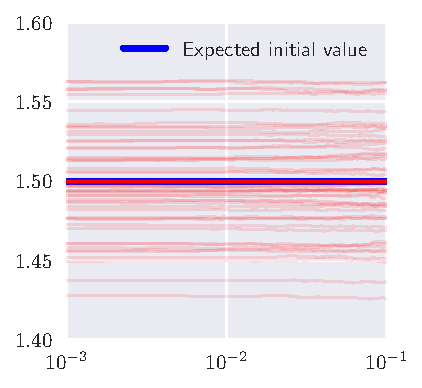
\includegraphics[width=1.\textwidth]{figures/risk_samples.pdf}
    \caption{samples estimation}
  \end{subfigure}
  \begin{subfigure}{0.495\textwidth}
    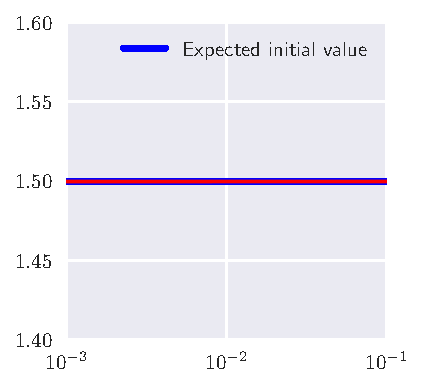
\includegraphics[width=1.\textwidth]{figures/risk_macroscopic.pdf}
    \caption{formula estimation}
  \end{subfigure}

  \caption{
    difference between two different strategies for estimating the risk in committee machine simulation.
    The two pictures are showing the same simulations and are zoomed on the very first part of the learning.
    There are 50 trajectories; we used 20000 samples for the estimation.
  }
  \label{fig:sampling_formula_risk}
\end{figure}

In Figure~\ref{fig:sampling_formula_risk} we show the difference between the last two strategies.
It's clear that the second one is preferable because the noise is reduced to 0, and the only difference
that appears in trajectories is caused by the stochasticity of the process.

\subsubsection{Finite size effect}
The key point of our analysis is the high dimensional limit; the derivation of 
deterministic differential equations are based on the limit \(d\to+\infty\).

When simulating a committee machine, we obviously can't use an infinite input layer dimension.
This introduces some finite-size effects. The simulations may not match exactly with the 
differential equations solution, but the difference becomes smaller and smaller by 
increasing the size used. 

This hypothetical problem has been a constant throughout this project,
although most of the time it has turned out not to be the cause of the discrepancies.
Many times we investigated the finite size effect, looking for a discrepancy scaling as
a power law (\(\propto d^\alpha\) for some \(\alpha\)), but we have not found any situation where
it was really affecting our results. Usually, \(d=10000\) was enough for our analysis; 
in the rest of this paper, we will not discuss this effect again assuming that
it is not relevant to what we are talking about, except where explicitly written.

% In Figure~\ref{fig:finite_size_example} we present an example of finite size effect;
% % todo: breve commento quando effettivamente metterai la figura.
% \begin{figure}
%   \begin{center}
%     \includegraphics[width=.7\textwidth]{example-image-duck}

%     \caption{
%       example of finite size effect. For details on how to interprete thi plot see Subsection~\ref{subsec:simulation_example}.
%     }
%     \label{fig:finite_size_example}
%   \end{center}
% \end{figure}

\subsection{Numerical solution of the differential equation}
The second ingredient needed for the numerical experiments of this work is a way to
solve the differential equations we derived in previous sections. Of course,
an explicit analytical solution is not feasible, given the complexity of the expressions;
we must therefore proceed with numerical integration techniques of differential equations. 

The most basic method for integrating a first-order differential equation is known
as \emph{Euler Method}, and it consists in discretizing the time in finite steps,
and compute the new value of the solution using the value at the previous step.
In our context, this becomes (let \(\delta t\) the time step)
\[
  \dod{\M{\left(t\right)}}{t} = \vec{\Psi}{\left(\vec{\Omega}\right)}
  \quad\xrightarrow{\text{Euler integration}}\quad
  \begin{cases}
    t^{(n)} = n \cdot \delta t \\
    \M^{(0)} = \M(0) \\
    \M^{(n)} = \vec{M}^{(n-1)} + \delta t\cdot\vec{\Psi}{\left(\vec{\Omega}^{(n-1)}\right)}
  \end{cases}\,.
\]
A completely analogous equation can be written for \(\Q\).

Of course, numerical integration introduces an error.
Since EM is a \emph{first-order method},
the error committed during the single step is proportional \(\delta t^2\).
Considering that the number of steps needed to reach a given time is inversely proportional
to the step size, the total error committed by this method of integration
is proportional to \(\delta t\).

For numerical experiments to be reliable, the error introduced by numerical integration
must be smaller (ideally negligible) than that due to switching from the stochastic process
to differential equations. Using the result of Theorem~\ref{thm:process_to_ode_goldt},
we get that the step size must satisfy
\[
  \delta t = \smallo{\frac{1}{\sqrt{d}}}\quad \text{ when }d\to+\infty.
\]
The usual choice for our numerical experiments is \(\delta t = \frac1d\);
this should ensure the negligibility condition respect the error of the Theorem.

\subsection{Example of a numerical experiment} \label{subsec:simulation_example}
\begin{figure}
  \begin{center}
    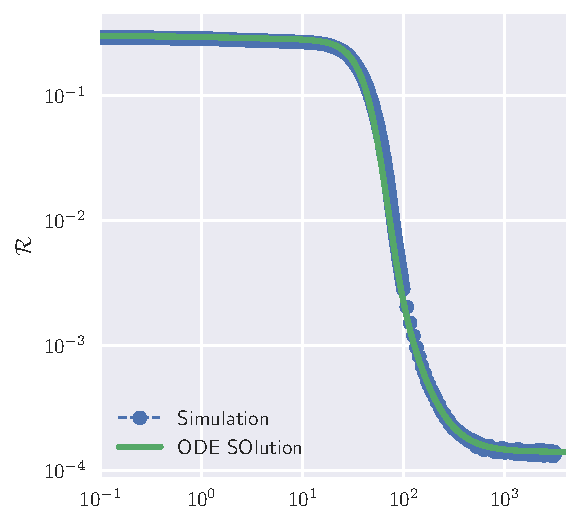
\includegraphics[width=.6\textwidth]{figures/simulation_examples_trajectory.pdf}

    \caption{
      the trajectory of both simulation and differential equations solutions in our example.
    }
    \label{fig:simulation_example_trajectory}
  \end{center}
\end{figure}
In this Section, we briefly present an experiment where we compare the simulation of committee machine training with the corresponding numerical simulation.
Although we do not present any results, we will use them to introduce some analysis tools that will be repeated in all future experiments.
We do not discuss the initial condition in this part since we will spend a lot of time on them in the next parts.

Let's start from the parameters used: \(d=1000, k=5, p=10, \gamma = 1., \Delta = \num{1e-3}, \delta t = \num{1e-3} \).
The only thing to be commented on here are the values of \(\Delta\) and \(\gamma/p\):
requiring the convergence of the process implies that they must not be too large;
we will derive precise inequalities in the sequel that will tell us exactly the maximum values that these two parameters can have.
For the moment, it is important to remember that they can be considered small enough to allow the second term of the equation for \(\Q\) to be considered at a lower order than the other terms of the ODEs.

Let's look at the plot of the risk through the process, in Figure~\ref{fig:simulation_example_trajectory}.
We use a logarithmic scale on both axes because we believe that's the best way to visualize what is going on in the process.
The simulation and solution trajectories of the differential equations match even though \(d\) is not very large;
this suggests that what has been exhibited so far is working. The simulated trajectory is subject to the noise introduced by the stochasticity of the training process,
so it will fluctuate around the trajectory defined by the solution of the differential equation. 
In the next Sections, we will often be interested in the transition between the initial flat phase and the onset of the fall (we call this transition ``drop from plateau'').
To make precise measurements in this area we will average several simulated trajectories in order to filter out the random part of the process.

To conclude, we present the analysis of the order parameter matrices, in Figure~\ref{fig:simulation_example_macroscopic}.
One important thing to say is that, given the symmetries, we discussed earlier,
it is sufficient to analyze the modulus of the matrix \(|\M\). 
We see from the figure that even starting from a completely uncorrelated state,
the dynamics found both student-teacher correlations and student-student correlations.
Truth be told, we will not report this kind of graph for our later experiments mainly for reasons of space.
Nevertheless, the usage of plots such as these was very helpful in the analysis of the model.
Although in the future we will only show plots of the kind in Figure~\ref{fig:simulation_example_trajectory},
it was not the only tool used for analysis.
\begin{figure}
  \centering
  \begin{subfigure}{0.495\textwidth}
    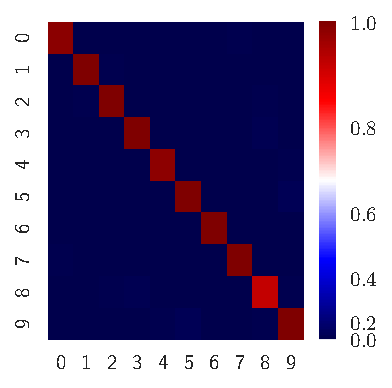
\includegraphics[width=1.\textwidth]{figures/simulation_examples_Q_start.pdf}
    \caption{\(\Q\) at start}
  \end{subfigure}
  \begin{subfigure}{0.495\textwidth}
    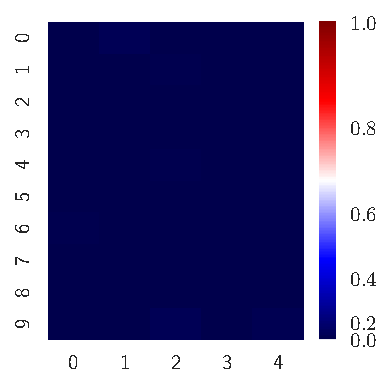
\includegraphics[width=1.\textwidth]{figures/simulation_examples_M_start.pdf}
    \caption{\(|\M|\) at start}
  \end{subfigure}
  \begin{subfigure}{0.495\textwidth}
    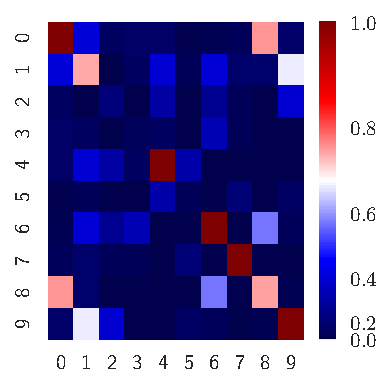
\includegraphics[width=1.\textwidth]{figures/simulation_examples_Q_end.pdf}
    \caption{\(\Q\) at end}
  \end{subfigure}
  \begin{subfigure}{0.495\textwidth}
    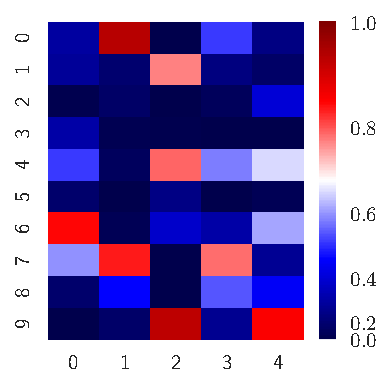
\includegraphics[width=1.\textwidth]{figures/simulation_examples_M_end.pdf}
    \caption{\(|\M|\) at end}
  \end{subfigure}

  \caption{
    order parameters matrix at the beginning and at the end of learning. 
  }
  \label{fig:simulation_example_macroscopic}
\end{figure}

Now that we know the tools we have available for analyzing an experiment, we can finally proceed with discussions about the content of the model.


\FloatBarrier
\section{Initial conditions}
In this Section, we present some considerations on the initialization of the student
and the teacher committee machines. As one may expect, the choice of the starting point 
can deeply affect the evolution of the training.
Moreover, we must always keep in mind that our ultimate goal is to give
an analytical estimate of the time required to learn the committee machine.
This forces us both to make a choice that produces analytically tractable equations
and to make a choice that is not too far removed from a real situation,
otherwise, the results would not be useful, despite being correct.

We initially present what was our first attempt to arrive at initial conditions suitable for our study.
Although it was not a fruitful choice,
we can still regard it as a toy model that serves as an introduction to the study of differential equations.
Next, we also report some other attempts, until we arrive at the final choice that we then used throughout our analysis.

\subsection{Symmetric initial condition} \label{subsec:symmetric_init}
Let's start by observing that form Equation~\eqref{eq:quadraticODE_M} it follows
that \(\M=0\) is a fixed point. This means that if we set completely non-overlapping
weights between student and teacher, then there is no learning at all, at least 
from the point of view of differential equations.
We would like to study the case where the teacher weights and the student's initial condition are uncorrelated,
and small perturbations around that. We introduce a framework where a parameter will
regulate the overlap, and the goal is doing perturbation around the fixed point.

The weights associated with a hidden node are vectors in \(\Real^d\), both for teacher and student.
Let \(\{\w^*_r\}_{r=1,\dots,k}\) the sets of weights of the teacher,
and \(V_T \coloneqq \Span\left[\{\w^*_r\}_{r=1,\dots,k}\right]\) the subspace generated by them.
We also assume these weights to be orthogonal. The initial weights for the student are chosen as
\[
    \w_j^0 = \frac{\varepsilon}{k} \sum_{r=1}^k \w^*_r + (1-\varepsilon) \w_j^S \quad
    \forall j\in [p],
\]
where the \(\w_j^S\) are orthogonal vectors of \(V_S \coloneqq (V_T)^\bot\),
the subspace of \(\Real^d\) orthogonal to the subspace of the teacher weights. 
The value of \(\varepsilon\) can vary between 0 and 1,
and it regulates the overlapping between student and teacher at the start.

We are using the following orthonormality conditions
\[
  \w^*_r \cdot \w^*_t = \rho_0d\delta_{rt}
  \qquad\text{and}\qquad
  \w_j^S\cdot\w_l^S=q_0d\delta_{jl},
\]
so the \emph{weights matrices} (\(\w_j \equiv [\W]_j\)) have orthogonal rows too.

Using all these assumptions, the computation of the order parameters leads to
\begin{align*}
  \left[\P\right]_{rt} &= \rho_0\delta_{rt}\\
  \left[\M^0\right]_{jr} &= \frac1d \w_j^0 \cdot \w^*_r = \frac{\rho_0\varepsilon}{k} \\
  \left[\Q^0\right]_{jl} &= \frac1d \w_j^0 \cdot \w^0_l = \frac1d
    \left(\frac{\varepsilon}{k} \sum_{r=1}^k \w^*_r + (1-\varepsilon) \w_j^S\right)\cdot
    \left(\frac{\varepsilon}{k} \sum_{t=1}^k \w^*_t + (1-\varepsilon) \w_l^S\right)\\
      &= \rho_0\frac{\varepsilon^2}{k} + q_0(1-\varepsilon)^2 \delta_{jl}
\end{align*}
An important feature of these initial conditions is that the order parameters are 
independent from \(d\), so the same differential equation solution can be used To
describe committee machines of different sizes.
Since what is really important is the rate between \(\rho_0\) and \(q_0\),
from now we will stick to the case \(\rho_0 = 1\).

\subsubsection{Fixed point with no overlap}
This case corresponds to null correlation, with \(\varepsilon=0\).
The initial conditions are 
\[\P = \I_k, \quad \M = 0 \quad \text{and}\quad \Q = q_0 \I_p.\]
As already pointed out, there is no evolution of \(\M\)
\[\M{(t)} = 0\quad \forall t\ge0,\]
and, through Equation~\eqref{eq:quadraticODE_Q},
this makes \(\Q\) always proportional to the identity matrix \(\Q{(t)} = q{(t)} \I_k\).
The important conclusion is that \(q(t)\) is the only variable that fully describes the evolution.
The equation Equation~\eqref{eq:quadraticODE_Q} becomes an explicit equation for \(q{(t)}\):
% ho rimosso tutti gli step perché non servono a niente. se proprio mettili in appendice
\begin{equation}\label{eq:eps0ODEforq}\begin{split}
    \dod{q{(t)}}{t} = \frac{4\gamma}{p}q{(t)}\Biggr\{\underbrace{
        1 - \left(1+\frac2p\right) q{(t)}}_{\eqqcolon L{(q{(t)};p)}}
    +\frac{\gamma}{p} \Biggr[\underbrace{
        \left(1+\frac2k+\Delta\right) - \Biggl(2 + \frac4p \Biggl)q{(t)} +
        \left(1+\frac6p+\frac{8}{p^2}\right)q^2{(t)}}_{\eqqcolon N{(q{(t)};p,k,\Delta)}}
    \Biggr]\Biggr\}.
\end{split}\end{equation}
We have introduced the two functions \(L\) and \(N\) in order to make the notation
lighter in the following part.

Since \(q(t)\) is descriptive of the whole process, we can write the population risk as its function
\[
  \risk{(t)} = \frac12\left[\left(1+\frac2k\right)-2q{(t)}+\left(1+\frac2p\right)q^2{(t)}\right].
\]
What it's really important about the last equation is that leads us to
\[
    \dod{\risk{(t)}}{t} = \left[\left(1+\frac2p\right)q{(t)}-1\right] \dod{q{(t)}}{t} = L{(q{(t)};p)} \dod{q{(t)}}{t},
\]
so stationary points of \(\od{q{(t)}}{t}\) are also stationary points of the risk itself, but the stability may be different.

Before continuing we show that \(L\) is always positive, regardless of the value of \(q\).
The function is a polynomial of the second degree,
so we have to show just that the (reduced) discriminant is less than 0
\[\begin{split}
  \left[-\left(1 + \frac2p \right)\right]^2 - \left(1+\frac6p+\frac{8}{p^2}\right)\left(1+\frac2k+\Delta\right) &<
  \left(1 + \frac2p \right)^2 - \left(1+\frac6p+\frac{8}{p^2}\right) \\
  &= 1 + \frac4p + \frac{4}{p^2} - 1-\frac6p-\frac{8}{p^2} 
  %=-(\frac2p+\frac{4}{p^2})
  <0.
\end{split}\]

We can now focus on the stationary and fixed points of the risk
since our ultimate goal is to have a description of its asymptotic behavior.
The first obvious fixed point is \(q=0\), but we are dealing only with positive values of \(q\),
so it's not interesting\footnote{
  We can show that if \(q{(0)}\) is positive, then we will never reach \(q=0\)
  by noticing that the time derivative of \(q\) is positive 
  in a right-neighborhood of \(q=0\).
}.
The second easy fixed point is the root of \(L{(q{(t)};p)}\):
\[q_{rm} \coloneqq \frac{1}{1+\frac2p} = \frac{p}{p+2}.\]
This corresponds to the minimum of the function \(\risk{(q)}\),
so it is not a real stationary point since the dynamic is governed by \(q\)
and this is not a fixed point for the \(q\) differential equation.

What really matters are the fixed points both for \(q\) and \(\risk\). 
Those are the roots of the equation obtained by imposing the left-hand-side 
of Equation~\eqref{eq:eps0ODEforq} equal to 0\footnote{
  We are assuming that solutions exist.
  If it not the case, then the problem is not interesting at all,
  since the risk will diverge independently from the value of \(q_0\).
}
\begin{equation}\begin{split}
  \displaystyle
  q_f^{1,2} &\coloneqq 
    \frac{p+2\gamma \mp
                \sqrt{\left[p+2\gamma\right]^2-
                      4\gamma p\frac{p+4}{p+2}
                        \left[1+\frac{\gamma}{p}\left(1+\frac2k+\Delta\right)\right]}}
                  {2\gamma\left(p+4\right)}p,
\end{split}\end{equation}

\begin{figure}
    \centering
    \begin{tikzpicture}[x=1.cm,y=1.cm,domain=0.:10.,range=-3.:5.]
      \filldraw [fill=Background,draw opacity=0.] (0,-3) rectangle (10.,5);
\draw[black, ->, thick] (0,0) -- (10,0) node[below] {\(q\)};
\draw[black, ->, thick] (0,-3) -- (0, 5) node[left] {\(\dod{q}{t}\)};

\draw (3,-0.15)--(3,0);
\draw (3.3,-0.15)--(3.3,0);
\draw (8,-0.15)--(8,0);

\draw[Blue, ultra thick] plot (\x,{0.4*(3-\x)});
\draw[Green, ultra thick] plot (\x,{0.1*(\x-3.3)*(\x-8)});

\draw[Red, dotted, thick] (3.3,0)--(3.3,1.5);
\draw[Red, dotted, thick] (3. ,0)--(3. ,1.5);
\draw[Red, |-|, ultra thick] (3. ,1.5) to node[Red,midway,above] {$\sim\BigO{\gamma}$} (3.3,1.5);

\node[above right] at (3.3,0) {$q_f^1$};
\node[below] at (3.,0) {$q_{rm}$};
\node[above] at (8,0) {$q_f^2$};
    \end{tikzpicture}
    \caption{
      the plot of the right-hand-side of Equation~\eqref{eq:eps0ODEforq}.
      The blue line is only the \(L\) contribution, while the green parabola is including also \(N\).
    }
    \label{fig:epsilon0stablepoints}
\end{figure}
To conclude our analysis, let us make a few considerations that will give us a clear picture
of how evolution works in this simple situation.
\begin{enumerate}
  \item \(q_f^1 < q_f^2\), by their definition;
  \item due to the fact that \(N{(q{(t)};p,k,\Delta)}\) is a positive function,
        the root of \(L{(q{(t)};p)}\) is always smaller than the full left-hand-side
        root in Equation~\eqref{eq:eps0ODEforq} (see also Figure~\ref{fig:epsilon0stablepoints} for a picture),
        so it holds\[q_{rm}<q_f^1 < q_f^2;\]
  \item As we already said, \(\risk{(q)}\) is a quadratic function and \(q_{rm}\) is the value of \(q\) that realize the minimum. Using previous step we can conclude
  \[\risk{(q_{rm})}<\risk{(q_f^1)} < \risk{(q_f^2)};\]
  \item We can show that \(q_f^1\) is a \emph{stable} point, while \(q_f^2\) is unstable (see Figure~\ref{fig:epsilon0stablepoints}).
  We can now infer the asymptotic behavior of the solution of the differential equation from the initial condition:
        \begin{itemize}
            \item \(0<q_0<q_f^2\): \(q{(t)}\to q_f^1\);
            \item \(q_0=q_f^2\): \(q{(t)}= q_f^2 \quad \forall t\);
            \item \(q_0>q_f^2\): \(q{(t)}\to +\infty\);
        \end{itemize}
        The interesting part comes from this initial value of \(q_0\):
        \[q_{rm}\le q_0<q_f^1 \quad \implies \quad \text{\(\risk{(t)}\) is a \textbf{strictly increasing} function}\]
        \[0\le q_0<q_{rm}     \quad \implies \quad \text{\(\risk{(t)}\) is a \textbf{non-monotonic} function}\]
  \item Let's look at the limit of small \(\gamma\):
        \[\lim_{\gamma\to0}q_f^1 = q_{rm} \quad\text{ and }\quad \lim_{\gamma\to0}q_f^2 = +\infty.\]
        This is in accordance with the common intuition that a smaller learning rate leads to better learning
        (even if talking about learning when there is no overlapping it's a little bit stretchy):
        we can go closer to the minimum and the interval where there is convergence is larger.
\end{enumerate}

We finally verified all our results from the study of differential equations with numerical experiments.
\begin{figure}
  \centering
  \begin{subfigure}{0.495\textwidth}
    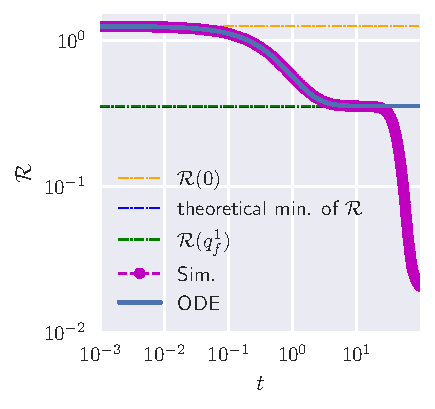
\includegraphics[width=1.\textwidth]{figures/example-eps0.pdf}
    \caption{global picture}
  \end{subfigure}
  \begin{subfigure}{0.495\textwidth}
    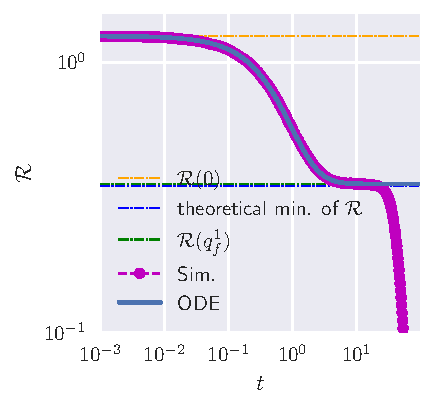
\includegraphics[width=1.\textwidth]{figures/example-eps0-zoomed.pdf}
    \caption{zoom}
  \end{subfigure}
  % Generated with: notebook epslion0
  \caption{
    example of a comparison between differential equations and simulations, with \(k=4\) and \(p=8\).
    The simulation and the analytic solutions match only in the first part.
    In Figure~(b) we zoom in on the region of the analytical prediction. We can see
    that the ODE solution converges to \(q_f^1\) and the theoretical risk minimum at \(q_{rm}\).
  }
  \label{fig:example-eps0}
\end{figure}
In Figure~\ref{fig:example-eps0} we show an example of a comparison between differential equations and simulations.
The first thing that stands out is that the simulations actually learn the teacher.
This happens because learning is a stochastic process, and the noise introduced
by the randomness of the SGD breaks the symmetry forced by the initial conditions.
On the other hand, the differential equations are deterministic, and their structure
is able to maintain the initial symmetry; the analytic solution gets stuck in the 
\emph{second plateau}. The only dynamics the ODE are able to catch in this case is 
the \emph{norm learning}: the weights of the student are changing their norm to adapt 
to the teacher, but their directions instead are not varying.

In the end, this section studied some initial conditions that do not bring out any kind of interesting learning.
In any case, the study of this simple toy model was useful to better understand the behavior of the dynamics of this strange activation function.
Finally, these particular initial conditions will be taken up in Chapter \ref{chap:stochasticity}.

\subsubsection{Overlapped intial condition}
We now generalize the study to the case \(\varepsilon\neq0\).
The initial conditions can be written as
\[\begin{split}
    \P &= \I_k,\\
    \M{(0)} &= \frac{\varepsilon}{k}\J_{p,k},\\
    \Q{(0)} &= \frac{\varepsilon^2}{k}\J_{p} + q_0(1-\varepsilon)^2\I_{p}.\\
\end{split}\]
We now show that \(\M\) and \(\Q\) stay in the same form through evolution, so we can write
\[\begin{split}
    \M{(t)} &= m{(t)} \J_{p,k} \\
    \Q{(t)} &= s{(t)} \J_{p} + q{(t)}\I_{p} \\
\end{split}\]
and the problem is completely described by a system of three coupled differential equations.
In order to prove this, it's sufficient the following identities
\[
    \I_d^n=\I_d, \quad \J_{d,f}^n = f^{n-1}\J_{d,f}, \quad \J_{d,f}\I_f = \J_{d,f}, \quad\text{and}\quad
    \J_{d,f} \J_{g,f}^\top = f \J_{d,g}.
\]
They are proof that the set \(\{\I,\J\}\) is closed under the operations that appear in differential equations.

The full derivation for the differential equations of \(m{(t)}\), \(q{(t)}\) and \(s{(t)}\) is 
omitted, since it's not particularly interesting. 

We avoided doing a careful study like the one in the previous section for the system of differential equations.
These initial conditions are not sufficiently general for a complete study of the learning process:
they still contain a symmetry that is preserved by the ODEs but broken from the 
stochasticity in the simulation. 
\begin{figure}
  \centering
  \begin{subfigure}{0.495\textwidth}
    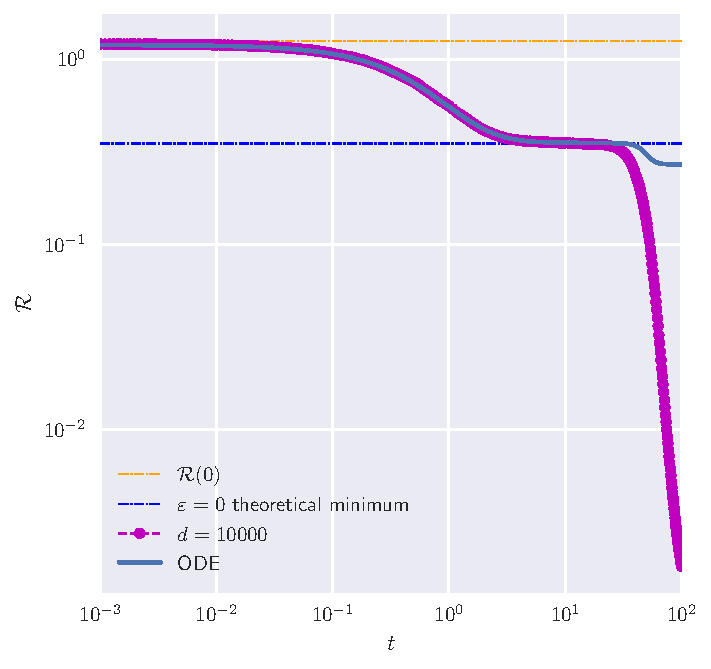
\includegraphics[width=1.\textwidth]{figures/example-small-eps.pdf}
    \caption{global picture}
  \end{subfigure}
  \begin{subfigure}{0.495\textwidth}
    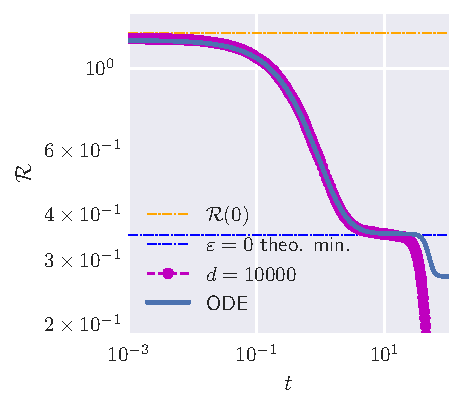
\includegraphics[width=1.\textwidth]{figures/example-small-eps-zoom.pdf}
    \caption{zoom}
  \end{subfigure}
  % Generated with: notebook small-epsilon
  \caption{
    example of a comparison between differential equations and simulations, with \(k=4\), \(p=8\) and \(\varepsilon=0.01\).
    The simulation and the analytic solutions match only in the first part.
    In Figure~(b) we zoom on the region of the analytical prediction.
    As in the previous case, the differential equations solution gets stuck in symmetry,
    while the simulation learns completely. The ``drop from the plateau'' happens before 
    the ODEs solution reaches its final value. 
  }
  \label{fig:example-small-eps}
\end{figure}

In Figure~\ref{fig:example-small-eps} we show an example of comparisons between simulation
and differential equation solution. The ODEs are now able to catch 2 different phases of 
the learning: the norm learning and the \emph{linear learning}. In the analytical dynamic,
they are clearly separated: the first part perfectly replicates what we saw in the previous section;
in the second part linear learning occurs, that is, each hidden neuron learns the same thing,
and the student's committee machine behaves as if \(p=1\).
This is evident from the fact that \(\M\) is proportional to \(\J\):
each hidden neuron is on average a copy of the others, they all learn the same weights.
In Figure~\ref{fig:pictorial-symmetric-learning} we present a schematic view of the different phases of the learning,
using symmetric initial conditions.
\begin{figure}
  \centering
  \begin{tikzpicture}[
    x=1.cm,
    y=1.cm
  ]
    \filldraw [fill=Background,draw opacity=0.] (0,0) rectangle (10.,9.);
\draw[black, ->, thick] (0,0) -- (10,0) node[below] {\(\log t\)};
\draw[black, ->, thick] (0,0) -- (0, 9) node[left] {\(\log\mathcal{R}\)};

\draw[
  line width=1.5mm,
  Red,
  looseness=1.1
] (0,8) to[out=0, in=180]
  (1.0,8) to[out=0, in=180]
  (2., 7) to[out=0, in=180] 
  (10, 7);

\draw[
  line width=1.mm,
  Blue,
  looseness=1.1
] (0,8) to[out=0, in=180]
  (1.0,8) to[out=0, in=180]
  (2., 7) to[out=0, in=180] 
  (4., 7) to[out=0, in=180]
  (5., 5) to[out=0, in=180]
  (10, 5);

\draw[
  line width=0.5mm,
  Green,
  looseness=1.1
] (0,8) to[out=0, in=180]
  (1.0,8) to[out=0, in=180]
  (2., 7) to[out=0, in=180] 
  (4., 7) to[out=0, in=180]
  (5., 5) to[out=0, in=180]
  (6., 5) to[out=0, in=180]
  (8., 1.5) to[out=0, in=180]
  (10., 1.5);

\node[right] at (1.5,7.55) {norm learning};
\node[left] at (4.5,6.) {linear learning};
\node[left] at (7.,3.25) {specialization};

\node[Red, above] at (9,7.05) {\(\varepsilon=0\)};
\node[Blue, above] at (9,5.05) {\(\varepsilon>0\)};
\node[Green, above] at (8.8,1.55) {\(\text{no symmetry}\)};

  \end{tikzpicture}
  
  \caption{
    pictorial representation of the different phases of learning for symmetric initial conditions.
  }
  \label{fig:pictorial-symmetric-learning}
\end{figure}

As already mentioned, simulations break this symmetry, and they do so before linear learning.
To be able to see the second plateau even in simulations would require using a much larger value of \(d\),
but this is not computationally feasible. 

We have empirically observed that in typical situations the various stages of learning are not really distinct and occur simultaneously,
so we decided to abandon symmetric initial conditions from here on,
in order to look for others that would suit us better.


\subsection{Random Initial condition} \label{subsec:random-initial-conditions}
In the last section, we have essentially come to the conclusion that
choosing initial conditions with some structure is convenient
because it simplifies the differential equations,
but it also introduces artificial symmetries that prevent the study of the complete problem.
We must therefore explore new possibilities to find ways to analyze the process of learning.

We decide to try some random initial conditions, to be sure that no symmetry is still present,
but at the same time use the high-dimensional limit to have statistical control on the 
order parameters. Moreover, we focus on the \emph{phase retrieval} case at first 
and then generalize once good initial conditions are found.
Accordingly, we will use the notation and the equations introduced in Section~\ref{subsec:phase_retrieval}.

We start our derivation by choosing both \(\vec{w}\) and \(\vec{w}^*\) to be independent normal
vectors with unit variance
\[
  w_{i}, w^*_{i} \sim \gauss{(0,1)}\quad\text{and all indipendent.}
\]
It follows that the order parameters are random variables too, distributed as
\emph{chi-squared} distribution
\[
  q(0),\rho \sim \frac{\chi^2_d}{d}
\]
and consequently 
\[
  \E\left[q(0)\right] = \E\left[\rho\right] = 1 \quad\text{and}\quad
  \Var\left[q(0)\right] = \Var\left[\rho\right] = \frac{2}{d}.
\]
The distribution of \(m{(0)}\) is not as simple as the previous two but can be derived exactly.
In our analysis it's sufficient to have the expected value and the variance, then use the 
\emph{central limit theorem} since we are interested in the high-dimensional limit.
Denoting \(X,Y\) two independent unitary normal variables, we can compute
\[\begin{split}
  \E\left[m{(0)}\right] =& \E\left[\frac{\sum_{i=1}^d w_iw^*_i}{d}\right] = \E\left[XY\right] = 0, \\
  \Var\left[m{(0)}\right] =& \Var\left[\frac{\sum_{i=1}^d w_iw^*_i}{d}\right]
    = \frac{1}{d^2}\sum_{i=1}^d \Var\left[XY\right] = \frac{1}{d}.
\end{split}\]
What emerges from these initial conditions is that, in the high-dimensional limit,
\(\vec{w}\) and \(\vec{w}^*\) are approximately two orthogonal vectors on the hemisphere of radius \(\sqrt{d}\).

The natural thing to do now is to replace these combined initial conditions with Equations~\eqref{eq:phase_retrieval},
with the aim of deriving approximate dynamics for the first part of learning
and to derive from it an analytical approximation of the learning time.
The problem is that is not clear how to do the approximation: an experiment reported in Figure~\ref{fig:unconstraned-random-example},
shows that \(q\) is varying considerably even before the learning starts.
This makes impossible all low-order expansions of differential equations and,
ultimately, analytical analysis of the phenomenon.
Nevertheless, in Figure~\ref{fig:unconstraned-random-m-exit-time} we show how an analysis of the simulations seems to suggest
a logarithmic trend in learning time as size changes. It is a crude numerical estimation of the behavior of the committee machine,
but it gives us a first idea of what is going on. To conclude, the behavior emerged from this analysis
is in accordance with what we may expect from past literature\cite{arous2021online}.
\begin{figure}
  \centering
  \begin{subfigure}{0.495\textwidth}
    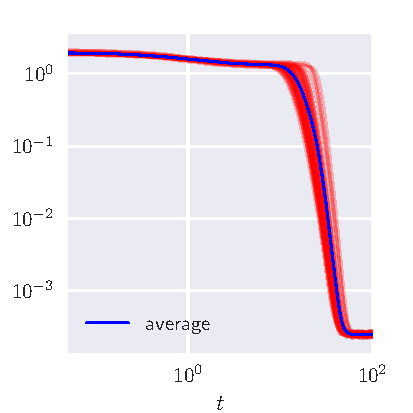
\includegraphics[width=1.\textwidth]{figures/unconstraned-phase-retrieval-risk.pdf}
    \caption{risk \(\mathcal{R}\)}
  \end{subfigure}
  \begin{subfigure}{0.495\textwidth}
    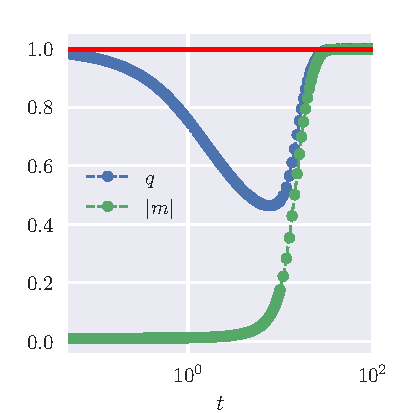
\includegraphics[width=1.\textwidth]{figures/unconstraned-phase-retrieval-qm.pdf}
    \caption{\(q\) and \(|m|\)}
  \end{subfigure}
  % Generated with: random-orthonormal-k=1
  \caption{
    example of simulation with random initial condition and \(d=10000\).\\
    In Figure~(a) we can see many different possible trajectories (red) and their average (blue).
    In Figure~(b) we plot the average of \(q\) and \(|m|\) over different trajectories.
    It's clear that the order parameter \(q\) is evolving considerably before the drop from initial
    plateau, so these initial conditions are not suitable for our goal.
  }
  \label{fig:unconstraned-random-example}
\end{figure}
\begin{figure}
  \centering
  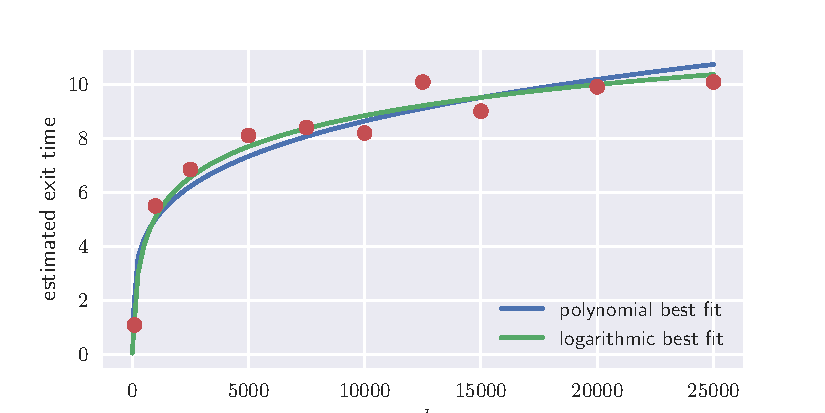
\includegraphics[width=\textwidth]{figures/unconstraned-phase-retrieval-exittimes.pdf}
  % Generated with: random-orthonormal-k=1
  \caption{
    plot of the \(|m|\) simulated exit time, and the corresponding best-fit curves.\\
    The exit time is estimated by measuring the time when the function \(m(t)\), averaged over many trajectories,
    crosses the threshold value \(0.1\).
    Looking at the figure, it is possible to convince oneself that 
    the logarithmic best fit better traces the behavior that emerged from the simulations. 
  }
  \label{fig:unconstraned-random-m-exit-time} 
\end{figure}
\FloatBarrier

In order to make the expansion possible, we have to set \(q(0)\) to be close to 0;
in other words, the norm of \(\vec{w}\) should be nearly null.
Obviously, we can't start exactly with \(\vec{w}=\vec{0}\), because it's a fixed point
of the differential equations dynamics.
Our goal can be achivied by intializing the student with \(w_{i}\sim\gauss(0,\sigma^2)\),
with \(\sigma^2\ll1\).
Recomputing the expected value above that are affected by this scaling of \(\vec{w}\), we get 
\[
  \E\left[q(0)\right] = \sigma^2\,, \quad
  \Var\left[q(0)\right] = \frac{2\sigma^2}{d}\quad\text{and}\quad
  \Var\left[m{(0)}\right] = \frac{\sigma}{d}. 
\]
The difference between these initial conditions and the previous one is illustrated in Figure~\ref{fig:pictorial-unconstrainted-phase-retrieval} .
\begin{figure}
  \centering
  \begin{tikzpicture}  
    % Credits to Nica 

% Sfera
\draw[turquoise, thick] (5,0) arc (0:180:5);

\fill[turquoise!33] (5,0) arc (0:180:5);

\draw[turquoise, thick, dashed] (0,0) ellipse (5 and 1.5);
\fill[turquoise!33] (0,0) ellipse (5 and 1.5);

% Vettori
\draw[black, ->] (0,0) -- (0,5) node[midway,right] {\(\vec{w}^*\)};

\draw[orange, ->] (0,0) -- (4,0.9) node[midway,above] {\(\vec{w}\)};

\draw[red, ->] (0,0) -- (-.8,0) node[midway,above] {\(\sigma^2\)};

\draw[loosely dashdotted, orange] (0,5) -- (4, 0.9);
\draw[gray] (0,0) -- (4, -0.9) node[midway,below]{$\sqrt{d}$};
\draw[loosely dashdotted, red] (0,5) -- (-.8,0);
  \end{tikzpicture}
  \caption{
    a pictorial plot of the phase retrieval weights with these initial conditions.
    The teacher weight, up to rotation, it's the pole vector in a semisphere 
    (here represented in 3D, but in the real case is \(d\)-dimensional);
    we can limit ourselves to analyzing only a hemisphere since the \(\vec{w}\to-\vec{w}\) symmetry applies.\\
    The two colored vectors represent the student's initial conditions, approximately orthogonal to the teacher vector. 
    The dashed lines are tentatives paths of the student vectors during the learning: starting close to the origin
    should make the norm grow towards~1, without any non-monotonic behavior.
  }
  \label{fig:pictorial-unconstrainted-phase-retrieval} 
\end{figure}
First of all, we observe that the sign of \(m(t)\) is not important for monitoring the learning. Therefore, the quantity
we are really interested in as initial condition is \(|m{(0)}|\). Using the \emph{half-normal distribution} properties\cite{enwiki:halfnormaldistribution},
we can compute
\[
  \E{\left[|m{(0)}|\right]} = \sqrt{\frac{2}{\pi d}}\sigma.
\]
We can now proceed to do a linear expansion of Equations~\eqref{eq:phase_retrieval} around the starting point
\begin{subequations}\begin{align}
  \dod{|m{(t)}|}{t} &= 6 \gamma |m{(t)}|\\
  \label{eq:sigma_phase_retrieval_q}
  \dod{q{(t)}}{t} &= \left(4 \gamma + 12 \gamma^2 + 4\Delta\right) q{(t)}
\end{align}\end{subequations}
where we transformed the equation for \(m(t)\) in the one for the modolus,
and kept only the linear terms of the equations\footnote{
  The expansion is not rigorous, since \(m(t)\) and \(q(t)\) are ``small'' for different reason.
  In order to do a proper derivation, we should keep track of different orders in different variables.
  The purpose of this part is to give an insight into what we will be doing in the next chapters.
}; we have also set \(\rho=1\), following what was computed above.
Using the expected values computed above as starting values, we get this evolution for the order parameters
\[
  |m(t)| = \exp{\left[6\gamma t\right]}\sqrt{\frac{2}{\pi d}}\sigma \quad\text{and}\quad
  q(t) = \exp{\left[\left(4 \gamma + 12 \gamma^2 + 4\Delta\right)t\right]}\sigma^2.
\]
We stress again that this evolution are approximating the real one only when \(m(t),q(t)\ll1\).
Despite this, we can still estimate exit times, provided the thresholds used are also small.
Let \(T\) the value of the threshold, valid both for \(m\) and \(q\), then the exit times are
\begin{equation}
  t_\text{ex}^{(m)} = \frac{\log{\left[\frac{T}{\sigma}\sqrt{\frac{\pi d}{2}}\right]}}{6\gamma} \quad\text{and}\quad
  t_\text{ex}^{(q)} = \frac{\log{\left[\frac{T}{\sigma^2}\right]}}{4 \gamma + 12 \gamma^2 + 4\Delta}.
\end{equation}
The thing to note is that \(t_\text{ex}^{(q)}\) does not depend on \(d\).
To make the result more accurate, we can make a correction to Equation~\eqref{eq:sigma_phase_retrieval_q}
and obtain a new form for the time evolution of \(q(t)\) that includes also the effect of \(m(t)\)
\[
  \dod{q{(t)}}{t} = \left(4 \gamma + 12 \gamma^2 + 4\Delta\right) q{(t)} + \left(8\gamma+48\gamma^2\right)m^2{(t)}.
\]
We can plug in the solution we found for \(|m(t)|\) and solve the equation to obtain\footnote{
  We are assuming that only \(m(t)\) can influence \(q(t)\) and that the reverse does not happen.
  This is not formally correct, but it is what happens in practice for reasonable choices of initial parameters.
}
\[\begin{split}
  q{(t)} = \frac{1}{8\gamma-12\gamma^2-4\Delta}\Bigg\{&\sigma^2\left[(8\gamma-12\gamma^2-4\Delta)-\left(8\gamma+48\gamma^2\right)\frac{2}{\pi d}\right]\exp\left[\left(4 \gamma + 12 \gamma^2 + 4\Delta\right)t\right]\\
          &+\left(8\gamma+48\gamma^2\right)\frac{2}{\pi d}\sigma^2 \exp\left[12\gamma t\right]\Bigg\}.
\end{split}\]
The evolution of q is contributed by two exponential;
it is not possible to derive an exact expression of the exit time,
but we can make the approximation that the two exponentials contribute separately
and thus take the minimum between the two possible times:
\[
  t_\text{ex}^{(q)} = \min\left(\frac{1}{4 \gamma + 12 \gamma^2 + 4\Delta}\log{\left[\frac{T}{\sigma^2}\right]},
                                \frac{1}{12\gamma}\log{\left[\frac{T}{\sigma^2}\frac{\pi d}{2}\frac{8\gamma-12\gamma^2-4\Delta}{8\gamma+48\gamma^2}\right]}\right),
\]
where we also dropped some subleading terms in \(d\).

Figure~\ref{fig:sigma-phase-retrieval-exittimes} shows a comparison between what is predicted by the formulas
and what is actually measured by doing the numerical experiments.
\begin{figure}
  \centering
  \begin{subfigure}{0.495\textwidth}
    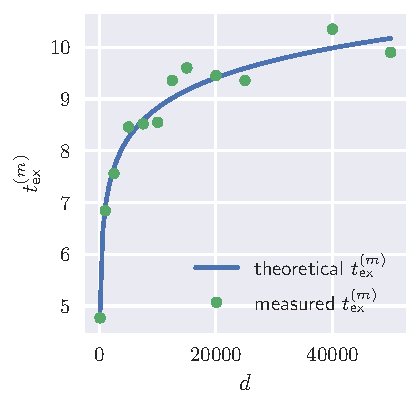
\includegraphics[width=1.\textwidth]{figures/sigma-phase-retrieval-mexit.pdf}
    \caption{exit time for \(|m|\)}
  \end{subfigure}
  \begin{subfigure}{0.495\textwidth}
    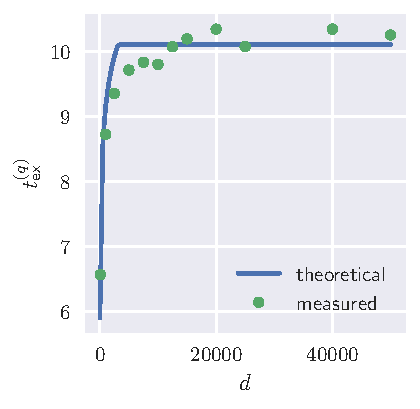
\includegraphics[width=1.\textwidth]{figures/sigma-phase-retrieval-qexit.pdf}
    \caption{exit time for \(q\)}
  \end{subfigure}
  % Generated with: random-orthonormal-k=1
  \caption{
    comparison between the exit time obtained from differential equations and the one measured in simulations. \\
    In the simulations we used \(\gamma=\num{0.1}, \sigma=\num{0.01}, T=\num{0.02}\).
  }
  \label{fig:sigma-phase-retrieval-exittimes}
\end{figure}
The predictions for \(t_\text{ex}^{(m)}\) are quite accurate,
while the ones for \(t_\text{ex}^{(q)}\) are only partially correct.
We can clearly see that our formula fails to predict the exit time in the transition
between the two regimes; probably the assumption that the two exponentials can be treated separately does not hold.
For large \(d\) the \(q\)-exit-time does not depend on \(d\) and the theoretical prediction seems correct.

The results obtained in this section, although not exhaustive,
provide an outline for what we are going to do in the next chapters of this paper.
The idea of random initial conditions combined with an expansion of differential equations seems promising,
but it has not yet led to the desired results.
The introduction of \(\sigma\) indeed made the expansion possible,
but it did not solve all the problems related to the norm of the \(\vec{w}\) vector;
it simply shifted the problem. 
The flat part in \(t_\text{ex}^{(q)}\)'s plot is a manifestation of the fact that the learning (linear or specialization) of the committee machine is still not being analyzed directly.
Achieving this goal will require a paradigm shift, as we will see in the next chapter.
